% !TeX program = PDFLaTeX
% !TeX encoding = UTF-8

\documentclass[letterpaper,12pt]{article}
% packages used
\usepackage{fullpage}
\usepackage{amsmath}
%\usepackage{amssymb}
%\usepackage{amsfonts}
\usepackage{amsthm}
\usepackage{bm}
\usepackage{graphicx}
\usepackage{cite}

% fonts used
%\usepackage{fourier}
\usepackage{fourier}
\usepackage{nimbusmononarrow}
\usepackage{microtype}
%\usepackage{fontspec}
%\setsansfont{Linux Biolinum}
%\setmonofont{Linux Mono}
% theorems, remarks, etc
  %% types italiques
\theoremstyle{plain}
\newtheorem{lemma}{Lemma}[section]
\newtheorem{proposition}{Proposition}[section]
\newtheorem{theo}{Theorem}[section]
\newtheorem{algo}{Algorithm}[section]
\newtheorem{assump}{\bf{Assumption}}[section]
\newtheorem{conj}{Conjecture}[section]
  %% types roman
\theoremstyle{remark}
\newtheorem{remark}{\bf{Remark}}[section]
\theoremstyle{remark}
\newtheorem{example}{\bf{Example}}[section]
\theoremstyle{remark}
\newtheorem{definition}{\bf{Definition}}[section]
  %\newtheorem{appendix}{\bm Definition}[section]


%------------------------------------------------------------------------
%--------------------------- personal macros ---------------------------
%------------------------------------------------------------------------

%\renewcommand{\theequation}{\arabic{section}.\arabic{equation}}
\numberwithin{equation}{section}

\newcommand*\diff{\mathop{}\!\mathrm{d}}
\newcommand*\Diff[1]{\mathop{}\!\mathrm{d^#1}}

%----- typos
\newcommand{\ie}{{\it i.e. \/}}

%----- fractions
\newcommand{\half}{\frac{1}{2}}

%---- bold characters
\newcommand{\bx}{{\bf{x}}}
\newcommand{\by}{{\bf{y}}}
\newcommand{\bk}{{\bf{k}}}
\newcommand{\bz}{{\bf{0}}}

%----- set
\newcommand{\R}{{\mathbb{R}}}
\newcommand{\Z}{{\mathbb{Z}}}
\newcommand{\N}{{\mathbb{N}}}
\newcommand{\Nm}{{\mathcal{N}}}
\newcommand{\RN}{\R^{\N}}
\newcommand{\p}{\mathcal{P}}

%----- derivatives
\newcommand{\dt}{\partial_t}
\newcommand{\dx}{\partial_x}
\newcommand{\dxx}{\partial_{xx}}
\newcommand{\dyy}{\partial_{yy}}
\newcommand{\dtt}{\partial_{tt}}
\newcommand{\dtx}{\partial_{tx}}
\newcommand{\dxtt}{\partial_{xtt}}
\newcommand{\dtxx}{\partial_{txx}}
\newcommand{\grdx}{\nabla_x}

\newcommand{\dz}{\partial_z}
\newcommand{\dnz}[1]{\partial^{#1}_z}

%----- greek letters
\newcommand{\eps}{\varepsilon}


%------------------------------------------------------------------------
%----------------------- end of personal macros ------------------------
%------------------------------------------------------------------------


\begin{document}

% \begin{flushright}
%   {\it draft, \today}
% \end{flushright}
%\begin{center}
\title{Notes}

\author{}
%\end{center}

\maketitle



\section{Introduction}
$dx = dy = 0.01$, $dt = 0.005$, $T = 1$. $r = 0.1$, $c = 50$, $D = 0.001$, $\rho = 10^{-12}$ and $\gamma = 0.75$.
\begin{figure}
  \includegraphics[width=0.5\textwidth]{1/m1}
  \includegraphics[width=0.5\textwidth]{1/s}
\end{figure}
\begin{figure}
  \includegraphics[width=0.5\textwidth]{1/PCG}
  \includegraphics[width=0.5\textwidth]{1/vector}
\end{figure}

\begin{figure}
  \includegraphics[width=0.5\textwidth]{2/m1}
  \includegraphics[width=0.5\textwidth]{2/s}
\end{figure}
\begin{figure}
  \includegraphics[width=0.5\textwidth]{2/PCG}
  \includegraphics[width=0.5\textwidth]{2/vector}
\end{figure}
\begin{figure}
  \includegraphics[width=0.5\textwidth]{3/m1}
  \includegraphics[width=0.5\textwidth]{3/s}
\end{figure}
\begin{figure}
  \includegraphics[width=0.5\textwidth]{3/PCG}
  \includegraphics[width=0.5\textwidth]{3/vector}
\end{figure}
\begin{figure}
  \includegraphics[width=0.5\textwidth]{4/m1}
  \includegraphics[width=0.5\textwidth]{4/s}
\end{figure}
\begin{figure}
  \includegraphics[width=0.5\textwidth]{4/PCG}
  \includegraphics[width=0.5\textwidth]{4/vector}
\end{figure}
\begin{figure}
  \includegraphics[width=0.5\textwidth]{5/m1}
  \includegraphics[width=0.5\textwidth]{5/s}
\end{figure}
\begin{figure}
  \includegraphics[width=0.5\textwidth]{5/PCG}
  \includegraphics[width=0.5\textwidth]{5/vector}
\end{figure}
\begin{figure}
  \includegraphics[width=0.5\textwidth]{6/m1}
  \includegraphics[width=0.5\textwidth]{6/s}
\end{figure}
\begin{figure}
  \includegraphics[width=0.5\textwidth]{6/PCG}
  \includegraphics[width=0.5\textwidth]{6/vector}
\end{figure}


\end{document}

